\documentclass{scrreprt}
\usepackage{paralist}
\usepackage{graphicx}
\usepackage[final]{hcar}

%include polycode.fmt

\begin{document}

\begin{hcarentry}{Simple San Simon Functional Web Browser (3S Functional Web Browser)}
\report{Carlos Gomez}
\status{experimental}
%\participants{(PARTICIPANTS OTHER THAN MYSELF)}% optional
\makeheader

Happy of me that I had the opportunity to work on a funcional programming project in my final project to get 
my Bachelor Degree in CS. Well, I have been experimenting building a Web Browser with Haskell.

It is called \textit{Simple San Simon Functional Web Browser} or just \textit{3S Functional Web Browser} 
(I honored the name of the University and the programming paradigm). As I mentioned before, I wanted to experiment some 
of the characteristics, libraries and tools of Haskell in the development of a Web Browser.\\

Some of those libraries and tools I have used were: \textit{libcurl} for obtaining the web resources, \textit{uu-parsinglib} 
for analysing HTML and CSS inputs, \textit{uuagc} for doing the transformations and computations and \textit{wxHaskell} for rendering web pages
and GUI.\\

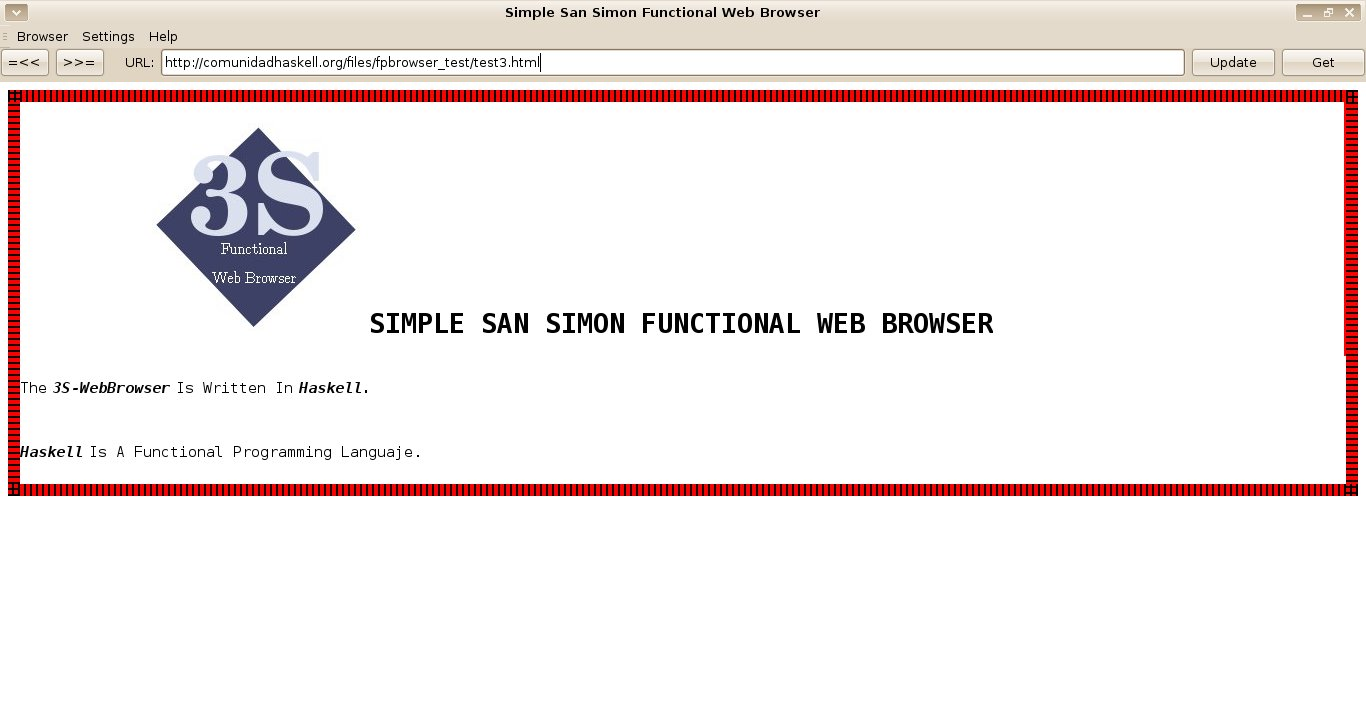
\includegraphics[scale=0.35]{img3sfwb.jpg}

As far I could reach developing, I give support to:
\begin{itemize}
    \item Working with HTTP and File protocols.
    \item A subset of the XHTML/XML grammar.
    \item A subset of the CSS grammar.
    \item 48 CSS properties, which let it:
        \begin{itemize}
            \item Modify the dimesion, position, type and style of an element.
            \item Modify the style of a text.
            \item Render list.
            \item Do content generation.
        \end{itemize}
\end{itemize}

I have to mention also that it has a lot of performance problems and lack of functionalities; Anyway, I have enjoyed a lot experimenting with it. 
I hope to have time to continue working on this.\\

Sources are on \url{https://github.com/carliros/Simple-San-Simon-Functional-Web-Browser}.

%\FurtherReading
%  \url{http://hsbrowser.wordpress.com}
\end{hcarentry}

\end{document}
